\documentclass[11pt,ngerman]{report}

\usepackage[a4paper, left=2cm, right=2cm, top=2cm, bottom=2cm]{geometry}
\usepackage[ansinew]{inputenc}
\usepackage[T1]{fontenc}
\usepackage[ngerman]{babel}
\usepackage[at]{easylist}
\usepackage{graphicx}
\usepackage{tabulary}
\usepackage{multirow}
\usepackage{booktabs}
\usepackage{hyperref}
\usepackage{acronym}
\usepackage{booktabs}

%\setlength\parindent{0pt}
\renewcommand{\baselinestretch}{1.5}

% Title Page
\title{Konzipierung und Implementierung eines geschwindigkeitsbasierten Reaktionsspiels unter Verwendung des 8051 Mikrocontrollers}
\author{Grundmann, Alexander; 5213081\\Köhler, Sven; 3158615\\Schneble, Adrian; 6418337\\Weickenmeier, Marc; 8724402}


\begin{document}

%%%%%%%%%%%%%%%%%%%%%%%%%%%%%%%%%%%%%%%%%%%%
\maketitle

%%%%%%%%%%%%%%%%%%%%%%%%%%%%%%%%%%%%%%%%%%%%
\tableofcontents


%%%%%%%%%%%%%%%%%%%%%%%%%%%%%%%%%%%%%%%%%%%%
\chapter{Einleitung}

\section{Motivation}

Im Zeitalter der Digitalisierung und des \ac{iot} werden Embedded Systems immer wichtiger. Da moderne objektorientierte Programmiersprachen wie bspw. C\# oder Python, aber auch prozedurale Sprachen wie C keine detaillierten Kenntnisse der Hardware erfordern, lernten wir in der Vorlesung ``Systemnahe Programmierung'' bei Herr Prof. Dr. Ralph Lausen hardwarenahe Entwicklung kennen. Insbesondere beschäftigten wir uns mit dem 8051 Mikrocontroller und dessen Programmierung.
Dementsprechendes Ziel dieses Projekts ist daher vorrangig der Einsatz des Controllers zur Erstellung eines Programms unserer Wahl.
In diesem Kontext wurde von uns demokratisch die Entwicklung eines geschwindigkeitsbasierten Reaktionsspiels beschlossen.


\section{Aufgabenstellung}

Ziel dieses Projekts ist die Entwicklung eines Programms für den 8051 Mikrocontroller unter Verwendung der MCU 8051 IDE, welche die Hardwarekomponenten simuliert.
Dies ermöglicht es, die Software ohne einen physisch vorhandenen Mikrocontroller schnell und wiederholt auszuführen.

Im Rahmen unseres Projekts entwickelten wir ein Geschwindigkeits-basiertes Reaktionsspiel. Wenn das Spiel beginnt, startet ein Timer, der nach einer zufälligen Zeit die linke oder rechte Hälfte des Displays ausschaltet. Ziel ist es, möglichst schnell die der jeweiligen Bildschirmseite entsprechenden Tasten zu betätigen. Je zügiger die Taste gedrückt wird, desto höher die Punktzahl.


% 4 Striche --> Taste wird gedrückt --> volles display --> Bildschirm geht auf einer Seite aus --> 

%%%%%%%%%%%%%%%%%%%%%%%%%%%%%%%%%%%%%%%%%%%%
\chapter{Grundlagen}

Um die nun erklärte Aufgabenstellung in die Tat umsetzen zu können müssen einige Grundlagen geklärt werden. Hierzu zählt der 8051 Mikrocomputer, die Assemblersprache und die verwendete Entwicklungsumgebung MCU-8051.

\section{Assemblersprache}

Eine Assemblersprache ist eine, auf eine bestimmte Prozessorarchitektur ausgerichtete, Programmiersprache. Sie wird als maschinenorientierte Sprache bezeichnet und löste die direkte Programmierung mit Zahlencodes ab. Dies hat den Vorteil, dass Operanden und Befehle durch mnemonische Symbole dargestellt werden können. Somit sind nun einfach lesbare Befehle wie “MOV” oder “ADD” möglich, welche jeweils genau einem Maschinenbefehl entsprechen.\footnote{http://www.carpelibrum.de/tutorials/einfuehrung\_in\_programmierung.pdf}
Dadurch kann und muss sehr hardwarenah (z.B. durch manuelle Register-Zugriffe oder CPU-Anweisungen) programmiert werden. Durch diese Nähe zur Hardware ist es ebenfalls möglich sehr Performance-orientiert zu programmieren, was bis ungefähr in die 1990er Jahre in der Computerspieleindustrie genutzt wurde. Hier mussten die Computerspiele möglichst performant laufen, da sonst kein flüssiges Spielen möglich war. Aus diesem Grund wurde hier noch lange auf Assemblersprachen gesetzt.
Auch in der heutigen Zeit wird in einigen Bereichen noch auf Assemblersprachen gesetzt. Dies geschieht vor allem bei sehr zeitkritischen Anwendungen oder in so genannten Embedded Systems (dt. Eingebettete Systeme), denen meist sehr wenig Speicherplatz zur Verfügung steht.

\section{Der 8051 Mikrocontroller}

Der 8051 Mikrocomputer ist ein Teil der MCS-51 Familie von Intel. Er besitzt 4096 Byte internen ROM und 128 byte internen RAM. Es wurden zwei 16-bit Timer verbaut.\footnote{https://www.mikrocontroller.net/articles/8051}

\begin{figure}[h]
	\caption{8051 Mikrocontroller}
	\centering
	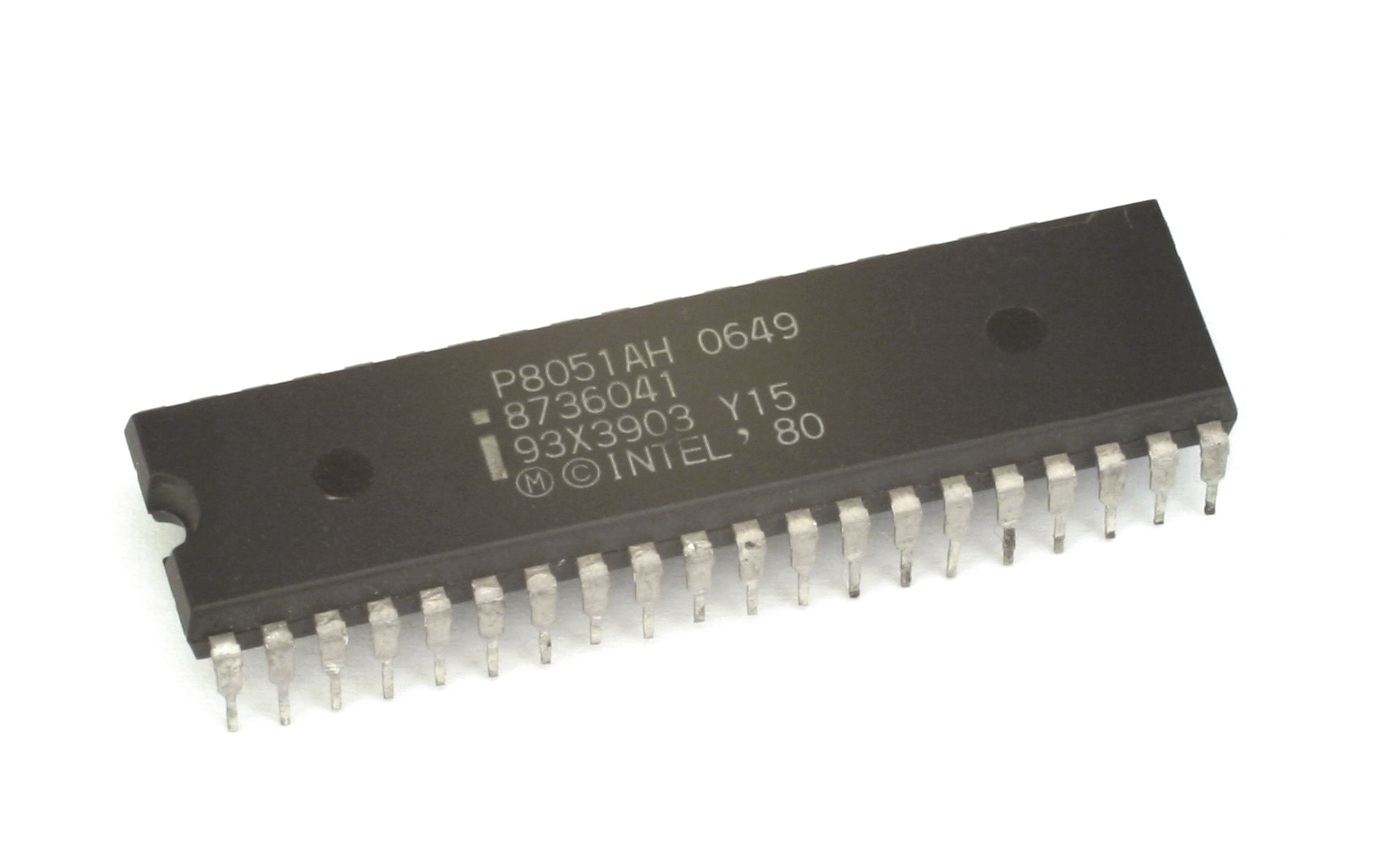
\includegraphics[width=\textwidth]{Prozessor.jpg}
\end{figure}

Für einen Befehl werden mindestens 12 Takte benötigt. Befehls- und Datenspeicher sind logisch getrennt.\footnote{https://www.mikrocontroller.net/articles/8051}

Ein Problem bei der Verwendung der Assemblersprache des 8051 Mikrocontrollers ist die eingeschränkte Auswahl an Befehlen. Beispielsweise sind die Befehle “JGT” oder “JLT” (Jump-Greater-Than / Jump-Less-Than), die in anderen Assemblersprachen vorhanden sind, für den 8051 nicht implementiert, sodass die Funktionalität zwar nicht eingeschränkt, aber komplizierter umzusetzen ist.

\section{Entwicklungsumgebung MCU-8051 IDE}

Eine Entwicklungsumgebung, auch \ac{ide} genannt, hilft Entwicklern beim Arbeiten mit der entsprechenden Programmiersprache und Plattform. Die in diesem Projekt genutzte MCU-8051 IDE wurde speziell für die Entwicklung von Mikrocontrollern ausgelegt, wozu auch der hier genutzte 8051 gehört. Hierzu kommt, unterstützend zur Entwicklung für möglichst reale Bedingungen, die integrierte Simulation von elektronischen Peripheriegeräten. Für die Anzeige von Daten bzw. Informationen werden LED-Panels, LED-Displays, LED-Matrizen, Multiplexed LED-Matrizen (4-stellige 7-Segment-Anzeige) oder ein LED-Display angeboten. Für die Eingabe, also Unterbrechung (Interrupt), stehen Bauteile wie Simple Keypads, Multiplexed Keypads, und ein Messgerät, den DS1260 temperature sensor. 

Diese virtuellen Bauteile können über den Menüreiter “Virtual HW” (Virtual Hardware) verwendet werden. Um diese Anzusteuern, müssen Pins (zur Verfügung stehen P0 bis P3 mit jeweils 8 Bit) mit den Bauteilen verknüpft werden.

\section{GitHub}

Um eine effektive Zusammenarbeit an dem Programmcode, sowie der Dokumentation gewährleisten zu können benutzen wir das Versionsverwaltungssystem GitHub.


%%%%%%%%%%%%%%%%%%%%%%%%%%%%%%%%%%%%%%%%%%%%
\chapter{Konzept}

\section{Idee}
Da nun die Grundlagen geklärt wurden, kann die Konzeption der Implementierung begonnen. Hierzu sollte zuerst die Idee genauer spezifiziert werden.
Das Reaktionsspiel startet mit vier Bindestrichen, die den Startzustand signalisieren. Es existieren zwei Buttons. Einer für die linke und ein weiterer für die rechte Seite der 4-stelligen 7-Segment Anzeige. Wird nun im Startzustand einer der beiden Buttons gedrückt, so startet das Spiel. Die Anzeige wird komplett gefüllt und es wird eine zufällige Zeit gewartet. Sobald diese Zeit abgelaufen ist, wird eine Seite der Anzeige ausgeschaltet. Nun muss der Button gedrückt werden, welcher sich noch auf der beleuchteten Seite befindet. Hat der Benutzer den richtigen Button gedrückt, so wird die benötigte Reaktionszeit in Millisekunden angezeigt. Bei einer falschen Eingabe geht das Programm in einen Fehlerzustand über, welcher durch 4 Bindestriche signalisiert wird. Nun kann, sowohl im Fehlerzustand, als auch in der Reaktionszeit-Anzeige, ein beliebiger Button gedrückt werden um das Spiel erneut zu starten.

\section{Voraussetzungen}
Für das Reaktionsspiel sind verschiedene Komponenten erforderlich. Unter anderem wird eine 4-stellige 7-Segment-Anzeige benötigt, die das Hauptdisplay darstellt. Des Weiteren werden 2 Eingabemöglichkeiten, bevorzugt Knöpfe, benötigt, die bspw. zum Starten des Spiels oder zum Reagieren auf die Zustandsänderung verwendet werden. Schlussendlich wird auch ein Timer benötigt, um die Zeit bis zum Anzeigen des Reaktionstriggers zu zählen und um Pseudozufallszahlen für die Auswahl der linken oder rechten Seite zu generieren.


\section{Programmentwurf}

Für den Programmentwurf werden verschiedene Zustände erstellt. Analog zu Kapitel 3.1 gibt es folgende Zustände: “statevoll”, “stateaktiv”, “statereagiert” und “statefehler”. “statefehler” stellt hierbei gleichzeitig den Start- und Fehlerzustand dar. Der gewünschte Programmablauf kann dem Programmablaufplan entnommen werden.

\begin{figure}[h]
	\caption{Programmablaufplan}
	\centering
	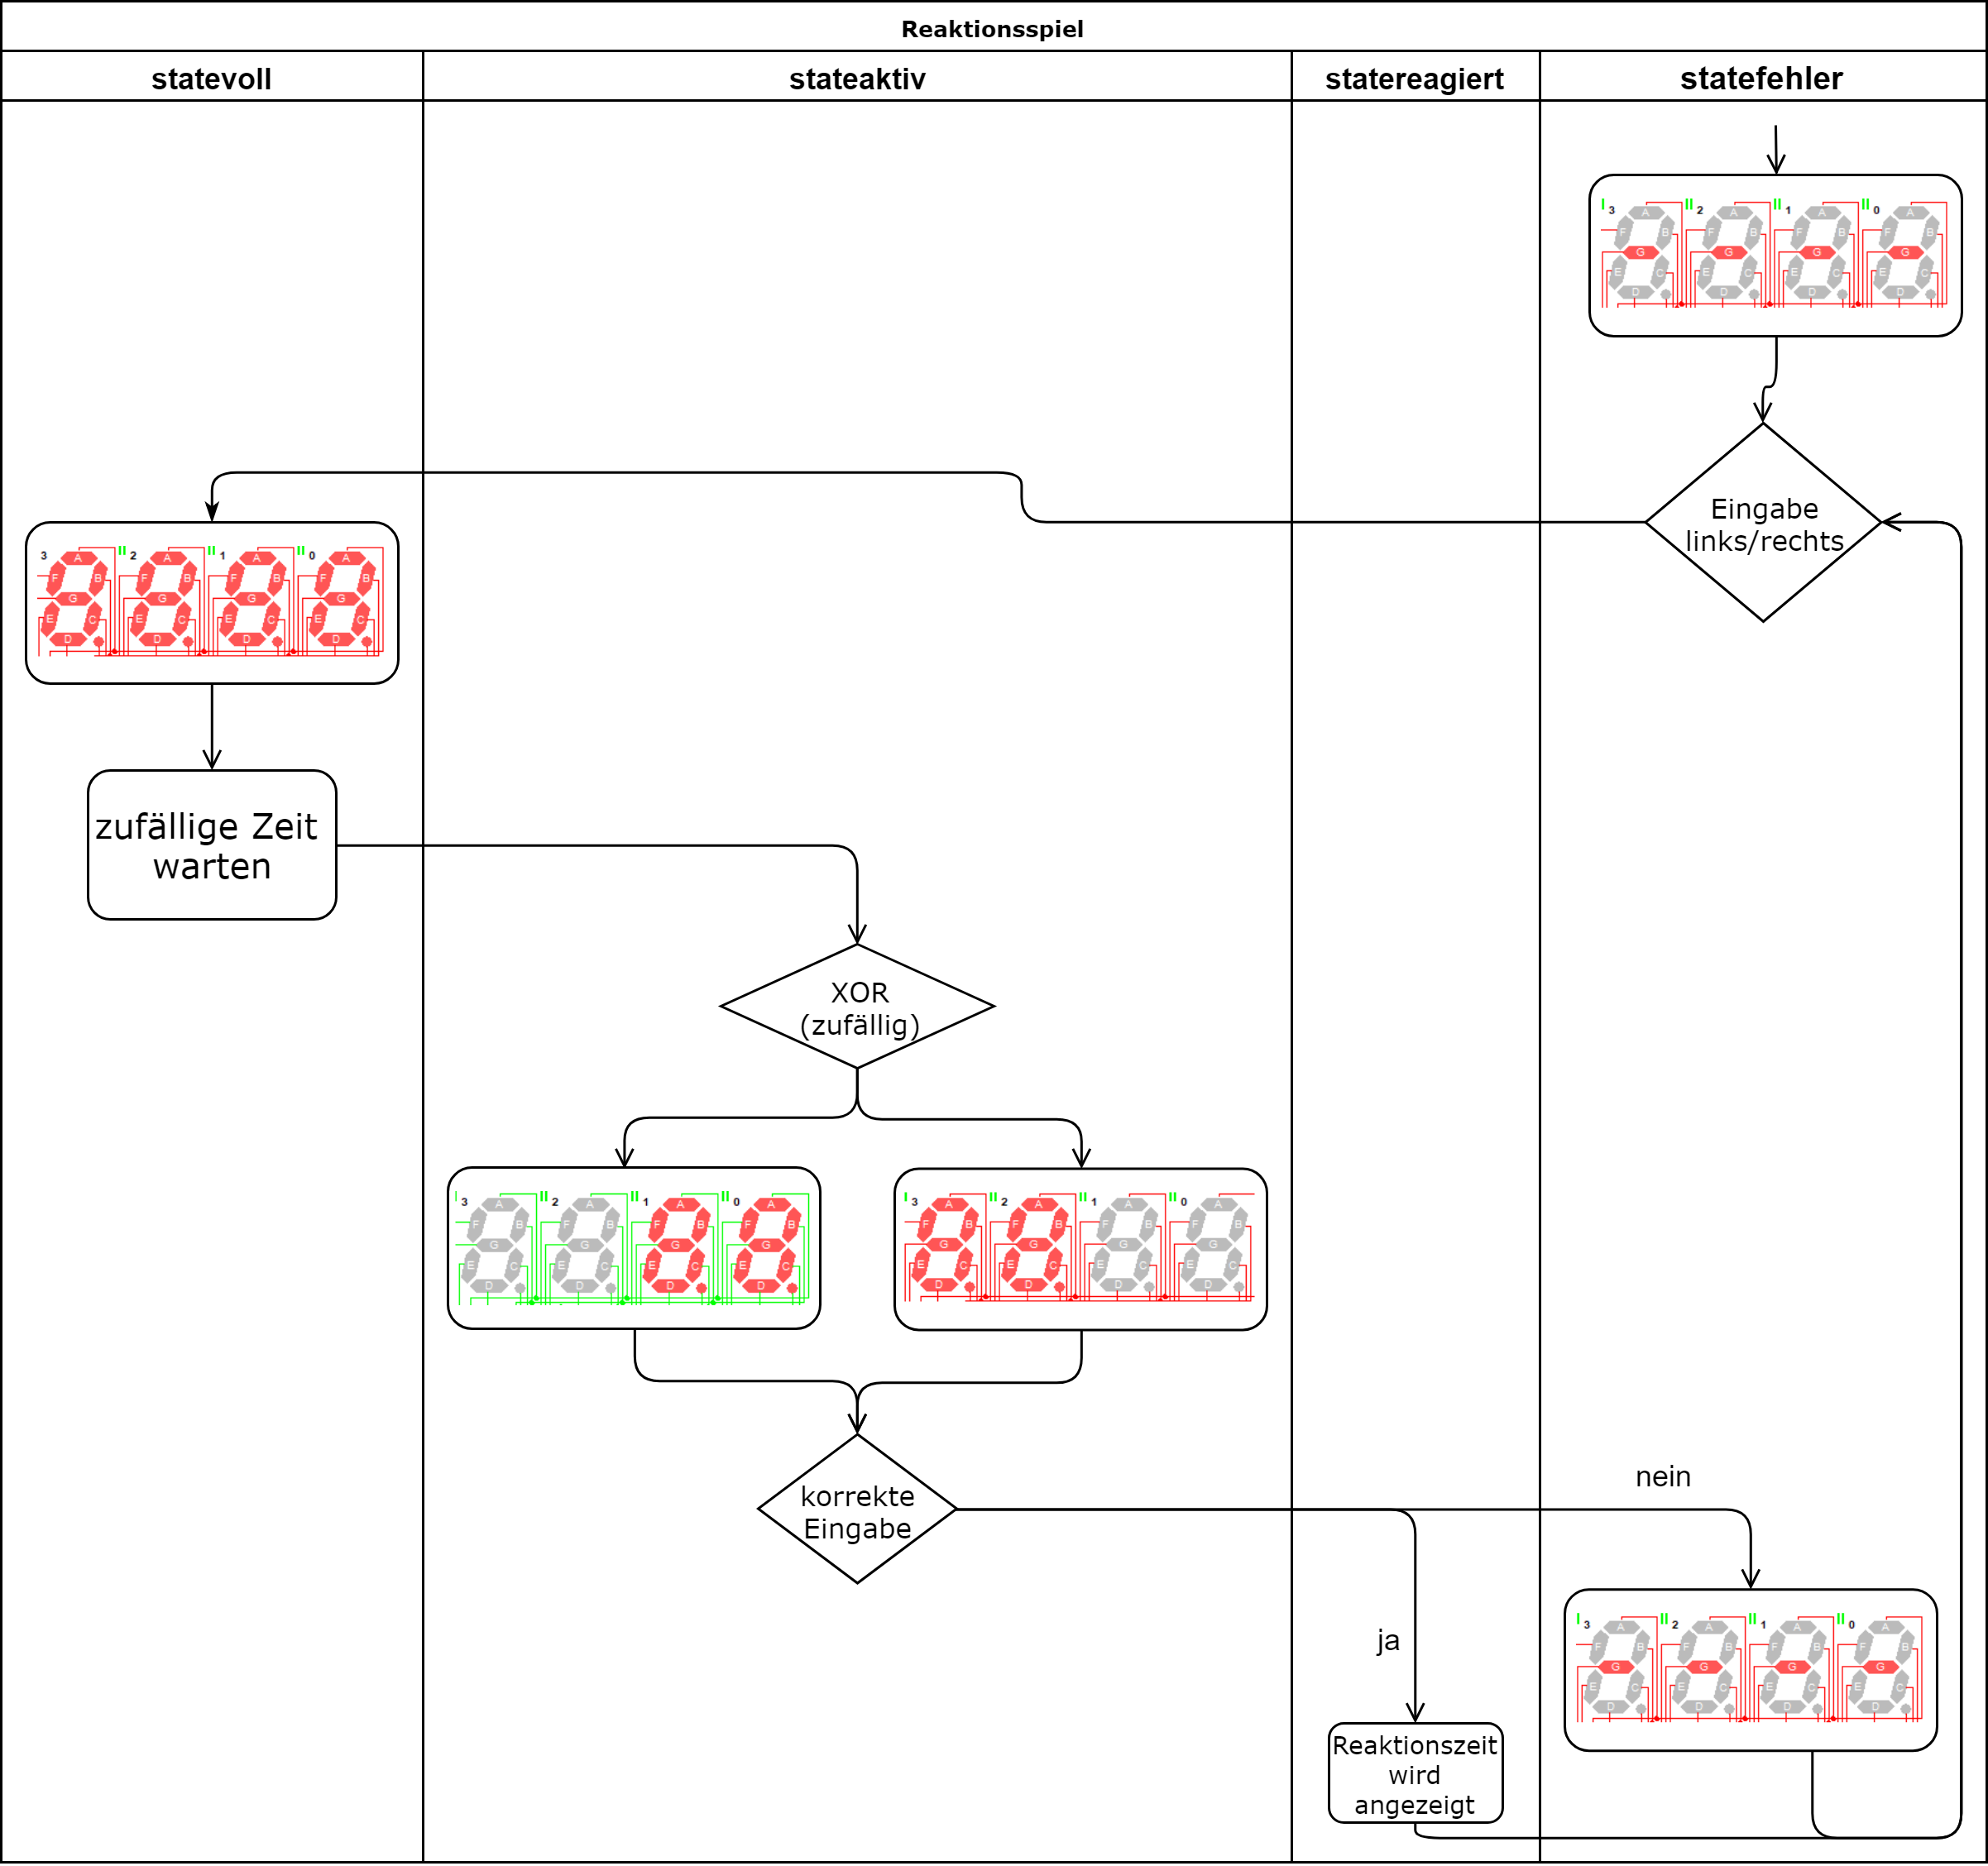
\includegraphics[width=\textwidth]{programmablaufdiagramm.png}
\end{figure}


%%%%%%%%%%%%%%%%%%%%%%%%%%%%%%%%%%%%%%%%%%%%
\chapter{Implementierung}

\section{Code}

Analog zu dem schon beschriebenen Programmentwurf soll nun die Implementierung des Reaktionsspiels beginnen. Zur Darstellung der Reaktionszeit wird eine Datenbank verwendet, in der die Ziffern Null bis Neun gespeichert und abgerufen werden können. Jeder Zustand wird durch eine Methode realisiert. Für das Auslesen der Reaktionszeit wird ein Timer verwendet. 
Zu Beginn des Progamms werden alle benötigten Werte initialisiert, der Timer gestartet, sowie eine erstes Zufallsbit berechnet. Dieses entscheidet später darüber, ob die linke, oder die rechte Seite aufleuchten soll.
\section{LED Matrix}

Zur Darstellung wird in diesem Projekt die virtuelle Variante eines Multiplexed LED Display verwendet, welches für die Darstellung der Spiel-Zustände und der Anzeige des Ergebnisses zum Spielende verwendet wird.

In folgendem Text wird die Funktionsweise der LED Matrix erläutert. Hierbei wird angenommen, dass die Pins P0 und P1 verwendet werden. Über die Bits 0 bis 3 des Pins P0 wird die zu verändernde 7-Segment Anzeige der LED Matrix festgelegt, wobei die Bits 0 bis 7 von P1 die anzuzeigende Ziffer darstellen.
Wird P0 auf den Binärwert 1111101 festgelegt, so wird die 7-Segment Anzeige angesprochen, die auf das vorletzte Bit (Position 1) festgelegt wurde - dies entspricht der letzten Anzeige (Position 1), welche in der folgenden Abbildung die Ziffer “6” anzeigt. Der Pin P1 wurde in diesem Fall mit dem Binärwert 10000010 belegt. Die Binärstellen stellen von Hinten nach Vorne gelesen die Abbildung auf die Segmente A-G der 7-Segment Anzeige und den Punkt dar. Hieraus ergibt sich folgende Tabelle für die benötigten Anzeigen:

\begin{table}[]
	\centering
	\caption{Binärtabelle für 7-Segment-Zahlen}
	\begin{tabular}{@{}ll@{}}
		\toprule
		Ziffer       & Binärwert \\ \midrule
		Leer-Zustand & 11111111  \\
		Minus (-)    & 10111111  \\
		Null (0)     & 01000000  \\
		Eins (1)     & 11111001  \\
		Zwei (2)     & 10100100  \\
		Drei (3)     & 10110000  \\
		Vier (4)     & 10011001  \\
		Fünf (5)     & 10010010  \\
		Sechs (6)    & 10000010  \\
		Sieben (7)   & 11111000  \\
		Acht (8)     & 10000000  \\
		Neun (9)     & 10010000  \\
		Voll (=8)    & 10000000  \\ \bottomrule
	\end{tabular}
\end{table}

Zur Anzeige mehrerer Stellen wird nun die Anzeige iterativ mit Zuständen versorgt. Durch die Anzeige-Verzögerung (z.B. 50ms) der Zeichen, bleiben zuvor gesetzte Zeichen weiterhin “aktiv”, leuchten also nach. Für jede 7-Segment Anzeige existiert ein zugehöriges Register, welches den Wert enthält. Im Hintergrund wird nun eine Routine dauerhaft ausgeführt, die jede Ziffer nacheinander setzt. Hierfür ist folgender Ablauf für jede Stelle notwendig (Beispiel anhand der ersten Stelle):

\begin{enumerate}
	\item Linke Ziffer aktivieren (P0 auf 11110111 setzen)
	\item Ziffernwert aus Register ziehen (R3 nach P1 kopieren)
	\item Ziffern-Ansteuerung resetten (P0 auf 11111111 setzen)
	\item Ziffernwert resetten (P1 auf 11111111 setzen)
\end{enumerate}

Das Zurücksetzen der Pins wird benötigt, um keine falsche “Beschriftung” der 7-Segment Anzeigen zu erzeugen. Sollte noch ein alter Wert auf Pin P1 anliegen, so wird beim wechseln der Ziffer (Pin P0) der vorherige Wert dargestellt. 

\begin{figure}[h]
	\caption{LED Display}
	\centering
	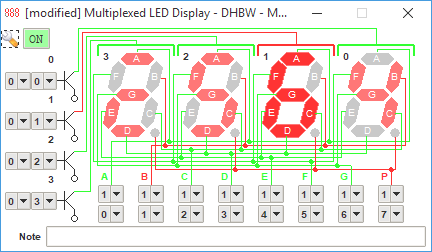
\includegraphics[width=\textwidth]{leddisplay.png}
\end{figure}


%%%%%%%%%%%%%%%%%%%%%%%%%%%%%%%%%%%%%%%%%%%%
\chapter{Fazit}
 
Die Implementierung des Projekts war ein Erfolg. Das Spiel kann somit gestartet und gespielt werden. Durch die eingeschränkte Performance der MCU-8051 Entwicklungsumgebung werden jedoch nicht die realen Reaktionszeiten angezeigt, da die Hardware nicht in Echtzeit simuliert werden kann. Sollte ein Anwender die reale Reaktionszeit messen wollen, so muss er das Programm auf echter Hardware, oder auf einer performanteren Entwicklungsumgebung installieren. Zu Testzwecken reichen die Daten der Simulation jedoch völlig aus. Schwierigkeiten bei der Entwicklung tauchten vor allem auf, wenn der Befehlssatz des 8051 nicht alle benötigten Funktionen umfasst. Ein Beispiel hierfür wären erweiterte Vergleichsoperatoren, wie größer oder kleiner. Dies konnte jedoch durch einige Zeilen Code gelöst werden.

%%%%%%%%%%%%%%%%%%%%%%%%%%%%%%%%%%%%%%%%%%%%

\newpage

\section*{Abkürzungsverzeichnis}

\begin{acronym}
	\acro{iot}[IoT]{Internet of Things}
	\acro{ide}[IDE]{Integrated Development Environment}
\end{acronym}

\end{document}          
